\documentclass[11pt]{article}
\usepackage[a4paper,margin=26mm]{geometry}
\usepackage[T1]{fontenc}
\usepackage{lmodern,microtype,amsmath,amssymb,amsthm,mathtools,booktabs,graphicx,array}
\usepackage[colorlinks=true,linkcolor=blue!45!black,citecolor=blue!45!black,urlcolor=blue!45!black]{hyperref}
\usepackage{xcolor,fancyhdr,enumitem}
\hypersetup{pdftitle={Gain-Aware Pole-Zero Cancellation on Protected Circles},pdfauthor={Shivam Gupta}}
\pagestyle{fancy}\fancyhf{}\fancyhead[L]{\small Gain-aware pole-zero cancellation}\fancyhead[R]{\small Shivam Gupta}\fancyfoot[C]{\thepage}
\setlength{\headheight}{14pt}
\newtheorem{theorem}{Theorem}[section]
\newtheorem{proposition}[theorem]{Proposition}
\newtheorem{corollary}[theorem]{Corollary}
\newtheorem{lemma}[theorem]{Lemma}
\theoremstyle{definition}\newtheorem{definition}[theorem]{Definition}
\newcommand{\C}{\mathbb C}\newcommand{\R}{\mathbb R}\newcommand{\eps}{\varepsilon}
\DeclareMathOperator{\conv}{conv}\DeclareMathOperator{\wind}{wind}
\title{Gain-Aware Pole-Zero Cancellation\\on Protected Circles\\[4pt]\large Sharp local errors, a common-gain obstruction,\\and exact budgeted matching}
\author{Shivam Gupta\\\small Independent Researcher\\\small \href{mailto:shivam1720406@gmail.com}{shivam1720406@gmail.com}\\\small ORCID: \href{https://orcid.org/0009-0009-4576-0138}{0009-0009-4576-0138}}
\date{17 October 2026}
\begin{document}\maketitle
\begin{abstract}
Removing a nearby pole and zero from a rational function is a geometric decision: Euclidean proximity alone does not control the change on an evaluation contour. We formulate cancellation as a relative approximation problem with an adjustable complex gain and one or more protected circles. Classical circle geometry gives the exact error for a proposed gain, and the best error on one circle is a pseudohyperbolic separation. For several circles, gain selection is a second-order cone problem. A convex-hull criterion characterizes when any common gain can achieve error below one, even when each circle separately permits a small error. Per-pair bounds yield a multiplicative budget; successive augmenting paths maximize the number of cancellations under that budget using exact rational comparisons. An independent verifier checks continuous-circle inequalities without optimization or boundary sampling. Experiments include 144 manufactured bank--budget cases and 36 nominal factorizations generated by noisy AAA fits. All 1,379 selected cancellations pass exact replay. At matched deletion counts, unprotected nearest-pair removal exceeds the tolerance in 37 manufactured cases. The method certifies change to a declared rational model; it neither identifies physical poles nor guarantees denoising or globally best rational compression.
\end{abstract}
\noindent\textbf{Keywords:} rational approximation; Froissart doublets; pole-zero cancellation; minimax approximation; validated computation; bipartite matching.\\
\textbf{MSC 2020:} 41A21, 65E05, 90C35.\\
\textbf{Software and measurements:} \url{https://github.com/shi1720/circlecancel}.

\section{Introduction}
A rational fit often contains a pole near a zero. Removing their factors reduces the degree and can suppress a narrow numerical artifact. The same operation can substantially change the function near a contour used for evaluation or singularity analysis. A cancellation policy should therefore answer a precise question: how much relative change is permitted on the declared evaluation set?

Consider a factor $(z-a)/(z-b)$ on the unit circle. With $a=1-\eta$ and $b=1-2\eta$, deleting it with unit gain changes the relative value by exactly one at $z=1$, however small $\eta>0$ becomes. An optimized gain reduces the worst change to $1/(3-2\eta)$, which still tends to $1/3$. Small Euclidean separation is insufficient even when both roots are inside the circle. If the roots straddle the circle, no nonzero gain achieves relative error below one.

This paper studies \emph{direct factor deletion}, retaining the other poles and zeros and allowing a constant replacement gain. This is distinct from deleting interpolation support points and refitting a new rational function. Our setting is useful when the retained factors must remain fixed, or when a proposed cleanup needs a simple, independently replayable error contract. Several circles can protect separate evaluation regions or both boundaries of an annulus. They must share the same replacement function and therefore the same gain.

The central observations are a complete common-gain feasibility criterion and an exact allocation procedure for the resulting error budget. The single-circle formula is an elementary consequence of M\"obius geometry and is presented as such. Our contributions are their specialization to a continuous relative-error cancellation contract; an example showing that separate-circle guarantees do not compose through independently chosen gains; exact maximum-cardinality matching for supplied rational edge certificates; and an implementation whose acceptance decision is checked by an independent, standard-library-only verifier.

\section{Related work and contribution boundary}
The AAA algorithm constructs adaptive barycentric rational approximations and includes a cleanup step for numerical Froissart doublets \cite{aaa}. Its support-deletion/refitting procedure can produce an excellent new fit; it does not preserve all remaining factors. SciPy exposes that workflow and a scale-aware cleanup test involving pole residues and nearby support points \cite{scipydoc}. These are relevant empirical comparators, not algorithms implementing our fixed-factor optimization problem.

Beckermann, Labahn, and Matos relate the absence of Froissart doublets to polynomial coprimeness, Sylvester-type conditioning, and spherical derivatives \cite{beckermann}. Their question concerns the numerical quality and separation properties of a rational representation. Here we take a declared factorization and ask which deletions satisfy a relative-error budget on specified circles. Trefethen's review explains the usefulness and sensitivity of rational analytic continuation and the limited effect that a near-canceling pair can have away from its location \cite{continuation}. Our analysis makes that dependence on an evaluation set explicit for direct cancellation.

Application-specific cleanup is also established. Yuan et al. remove a selected partial-fraction contribution from a Loewner-based fit to electromagnetic scattering data \cite{yuan}. Commercial control software provides tolerance-based pole-zero simplification \cite{minreal}. Neither the existence of cleanup software nor its commercial usefulness implies that the present method has been validated in a production engineering workflow.

Second-order cone programming \cite{boyd} and minimum-cost flow \cite{flows} are established tools. We use them without claiming a new general optimization algorithm. The exact-arithmetic implementation replaces sums of logarithms by rational products. The proposed research contribution is the complete cancellation interface: sharp geometric edge costs, a shared-gain obstruction, budgeted selection, and independent continuous verification. The literature reviewed did not identify this full formulation. That search cannot establish universal priority over unpublished or unindexed work.

\begin{table}[t]\centering\small
\caption{Scope relative to the closest lines of work. All entries concern the stated methods, not every possible extension of them.}
\begin{tabular}{p{.24\linewidth}p{.34\linewidth}p{.33\linewidth}}\toprule
Line of work & Main object & Distinction in this paper\\\midrule
AAA cleanup \cite{aaa,scipydoc} & Remove support points and refit & Direct factor deletion with retained factors fixed\\
Doublet diagnostics \cite{beckermann} & Conditioning, coprimeness, spherical derivative & Declared-circle relative change after deletion\\
Loewner cleanup \cite{yuan} & Selected partial-fraction removal & Common gain over multiple circles\\
Min-cost flow \cite{flows} & Minimum additive cost at fixed flow & Rational product comparisons for verified error costs\\\bottomrule
\end{tabular}\label{tab:prior}
\end{table}

\section{A relative-error cancellation contract}
Let $\Gamma_\ell=\{z:|z-c_\ell|=R_\ell\}$, $R_\ell>0$, and let $K=\bigcup_{\ell=1}^L\Gamma_\ell$. The circles may overlap or nest. Consider a nonzero rational function with a declared factorization
\begin{equation}
 r(z)=\kappa\frac{\prod_{i=1}^{n}(z-a_i)}{\prod_{j=1}^{m}(z-b_j)},\qquad \kappa\ne0.\label{eq:factor}
\end{equation}
Repeated factors are allowed. No listed root lies on $K$. A matching $M\subseteq\{1,\ldots,n\}\times\{1,\ldots,m\}$ uses each zero and pole at most once. Replacing each selected factor $(z-a_i)/(z-b_j)$ by a nonzero gain $\gamma_{ij}$ gives
\begin{equation}
 \frac{\widetilde r(z)}{r(z)}=\prod_{(i,j)\in M}\gamma_{ij}h_{ij}(z),\qquad
 h_{ij}(z)=\frac{z-b_j}{z-a_i}.\label{eq:ratio}
\end{equation}
The quotient is understood by its factor expression wherever removable cancellations occur. The required bound is
\begin{equation}
 \sup_{z\in K}\left|\frac{\widetilde r(z)}{r(z)}-1\right|\le E.\label{eq:contract}
\end{equation}
A small $E$ bounds multiplicative change, not error to an unknown target. It also does not preserve the individual pole or zero count inside a circle: deleting an inside pair removes one of each. Under a strict bound below one, the net count of zeros minus poles is preserved.

\subsection{Exact one-pair geometry}
Fix a zero $a$, a pole $b$, and a circle $(c,R)$, and abbreviate $A=a-c$, $B=b-c$. Define
\begin{equation}
 D=R^2-|A|^2,\qquad
 m=\frac{R^2-B\overline A}{D},\qquad
 s=\frac{R|a-b|}{|D|}.\label{eq:disk}
\end{equation}
The boundary hypothesis gives $D\ne0$.

\begin{lemma}[Image circle and exact error]\label{lem:image}
For $h(z)=(z-b)/(z-a)$ and any $\gamma\in\C$,
\begin{equation}
 \max_{|z-c|=R}|\gamma h(z)-1|=|\gamma m-1|+|\gamma|s.\label{eq:error}
\end{equation}
\end{lemma}
\begin{proof}
If $a=b$, then $h\equiv1$, $m=1$, and $s=0$. Otherwise set $w=h(z)$ and solve $z-c=(wA-B)/(w-1)$. The circle equation becomes $|wA-B|^2=R^2|w-1|^2$. Completing the square gives $|w-m|=s$, with \eqref{eq:disk}. The map traces the full image circle, so the greatest distance from $1$ after multiplication by $\gamma$ is the distance to its center plus its radius.
\end{proof}

\begin{theorem}[Best gain on one circle]\label{thm:single}
If $a,b$ lie on the same side of $\Gamma$, the unique best gain is $\gamma_*=1/m$ and the minimum error is
\begin{equation}
 \delta_\Gamma(a,b)=\frac{s}{|m|}
 =\frac{R|a-b|}{|R^2-(b-c)\overline{(a-c)}|}<1.\label{eq:pseudo}
\end{equation}
If they lie on opposite sides, the infimum over nonzero gains is one. Allowing the zero gain attains that value, but the zero function is not an admissible cancellation.
\end{theorem}
\begin{proof}
One has
\begin{equation}
 |m|^2-s^2=\frac{R^2-|B|^2}{R^2-|A|^2}.\label{eq:sides}
\end{equation}
For $m\ne0$, write $t=|\gamma m|$ and $\rho=s/|m|$. Equation \eqref{eq:error} is at least $|t-1|+\rho t$, with equality when $\gamma m$ is nonnegative real. If $\rho<1$, the unique minimum is at $t=1$, giving \eqref{eq:pseudo}. If $\rho>1$, the minimum with zero gain allowed is at $t=0$. Equation \eqref{eq:sides} determines these two cases. When $m=0$, the objective is $1+s|\gamma|$, with the same infimum one.
\end{proof}

For two roots inside the circle, \eqref{eq:pseudo} is the classical pseudohyperbolic separation after translating and scaling to the unit disk. Reflection $z\mapsto R^2/\overline{z-c}$ gives the corresponding exterior interpretation. The formula is invariant under common translations, rotations, and nonzero changes of scale. It is therefore preferable to an absolute Euclidean threshold when evaluation geometry changes.

\begin{proposition}[Arbitrarily fine finite validation can miss a fixed error]\label{prop:sample}
For every finite set $Z\subset\{|z|=1\}$ and $\tau>0$, a same-side pair exists for which unit-gain deletion has change at most $\tau$ on $Z$ and worst change exactly one on the whole circle. Its best-gain error tends to $1/3$ along the construction.
\end{proposition}
\begin{proof}
Choose $\zeta$ on the circle outside $Z$, and put $a=(1-\eta)\zeta$, $b=(1-2\eta)\zeta$, $0<\eta<1/2$. Then $|h(z)-1|=\eta/|z-a|$. At $z=\zeta$ this is one, its maximum because $\operatorname{dist}(a,\Gamma)=\eta$. At every point of $Z$ it tends to zero as $\eta\downarrow0$. Formula \eqref{eq:pseudo} gives $1/(3-2\eta)$.
\end{proof}

\section{One gain for several circles}
For each circle form $(m_\ell,s_\ell)$ using \eqref{eq:disk}. Its closed image disk is $D_\ell=\{w:|w-m_\ell|\le s_\ell\}$. Although $h$ traces the boundary, maxima of the absolute affine expression are the same over the disk. Thus the ideal joint error is
\begin{equation}
 \delta_K=\min_{\gamma\in\C}\max_{1\le\ell\le L}
       \bigl(|\gamma m_\ell-1|+s_\ell|\gamma|\bigr).\label{eq:joint}
\end{equation}
Writing $\gamma=x+iy$, multiplication by $m_\ell$ is a real $2\times2$ linear map. The epigraph inequalities in \eqref{eq:joint} are sums of Euclidean norms, hence admit a second-order cone formulation \cite{boyd}. Zero gain gives the upper bound one. A returned nonzero gain is useful only when its verified error satisfies the requested budget.

\begin{theorem}[Common-gain obstruction]\label{thm:hull}
Let $S=\bigcup_\ell D_\ell$. Then
\begin{equation}
 \delta_K<1\quad\Longleftrightarrow\quad 0\notin\conv S.\label{eq:hull}
\end{equation}
Consequently, putting both roots on the same side of every protected circle is necessary but not sufficient for a common gain with error below one.
\end{theorem}
\begin{proof}
If $0\in\conv S$, express zero as a convex combination of points of $S$. Convexity of $w\mapsto|\gamma w-1|$ gives $1\le\max_{w\in S}|\gamma w-1|$ for every gain.
Conversely, $S$ is compact. If zero is outside its compact convex hull, strict separation gives a complex $v$ and $\alpha>0$ with $\Re(vw)\ge\alpha$ for every $w\in S$. Let $\beta=\max_{w\in S}|vw|^2>0$. For $0<t<2\alpha/\beta$,
$|tvw-1|^2\le1-2t\alpha+t^2\beta<1$ uniformly on $S$. The nonzero gain $tv$ therefore has error below one. If a pair straddles a circle, \eqref{eq:sides} puts zero inside its image disk, proving necessity of the side condition.
\end{proof}

\paragraph{A strict incompatibility example.}
Take $a=0$, $b=1$, and two circles with centers $-0.1,0.1$ and common radius $0.01$. Both roots are outside both circles. Their individual best errors are approximately $0.0909918$ and $0.110988$. The image centers have opposite real signs; the segment joining them contains zero. Thus \eqref{eq:hull} gives joint optimum exactly one. Taking the larger of the individual errors would incorrectly declare a common error below $0.12$. The issue is the differing normalization, not topology alone (Figure~\ref{fig:geometry}).

\begin{figure}[t]\centering
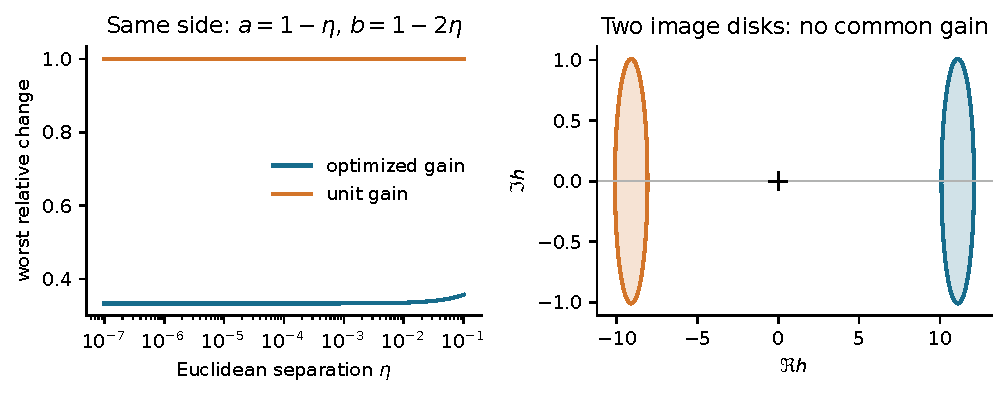
\includegraphics[width=\linewidth]{figures/geometry.pdf}
\caption{Left: Euclidean separation tends to zero while the optimized relative error stays near $1/3$; unit gain has error one. Right: image disks for the two-circle example. Each permits a good individual gain, but their convex hull contains zero, precluding any common gain with error below one.}\label{fig:geometry}
\end{figure}

\section{Composing errors and selecting cancellations}
Suppose each candidate edge $e=(i,j)$ has a nonzero gain and a verified bound
\begin{equation}
 \sup_{z\in K}|\gamma_e h_e(z)-1|\le\eps_e,\qquad 0\le\eps_e<1.\label{eq:edge}
\end{equation}
These may be conservative rational bounds for numerical gain proposals; ideal optimizer values are not required.

\begin{theorem}[Multiplicative error budget]\label{thm:product}
Every matching $M$ satisfies
\begin{equation}
 \sup_K\left|\frac{\widetilde r}{r}-1\right|
 \le \prod_{e\in M}(1+\eps_e)-1.\label{eq:product}
\end{equation}
This bound is sharp as a universal statement depending only on the per-factor errors. If its right-hand side is below one, $r$ and $\widetilde r$ have equal winding number about zero on each protected circle.
\end{theorem}
\begin{proof}
Write $\gamma_eh_e=1+u_e$ and expand the product minus one. Bounding each nonempty product by the corresponding product of $\eps_e$ proves \eqref{eq:product}. For sharpness, take $k$ identical factors with multiplicity and use their optimal single-circle gain. The error $u$ traces a circle centered at zero, so some common boundary point has $u=\delta>0$. The product error there equals $(1+\delta)^k-1$.
For the winding statement, $\widetilde r/r$ lies in a disk centered at one of radius below one. Its boundary path is homotopic to the constant one through nonzero values, so its winding is zero. Additivity of winding gives the conclusion.
\end{proof}

\begin{corollary}[Extension to a pole-free region of the quotient]\label{cor:region}
Let $\Omega$ be a bounded domain whose boundary consists of protected circles. If no removed zero lies in $\overline\Omega$, the bound \eqref{eq:product} holds throughout $\overline\Omega$. For a disk of radius $R$, the quotient $Q=\widetilde r/r$ also satisfies $|Q^{(k)}(z)|\le k!E/(R-r)^k$ for $|z-c|\le r<R$, whenever the boundary bound is $E$.
\end{corollary}
\begin{proof}
The factor formula makes $Q-1$ analytic on a neighborhood of $\overline\Omega$. Apply the maximum-modulus principle and then the Cauchy derivative estimate on disks of radius approaching $R-r$.
\end{proof}

This extension fails when a removed zero is inside the region: the quotient then has a pole there, even if deletion is safe on its boundary. The protected-set declaration is therefore part of the result.

\subsection{Exact maximum cardinality for the supplied budget}
Set $w_e=\log(1+\eps_e)$ and $B=\log(1+E)$. Maximizing $|M|$ under \eqref{eq:product} is equivalent to maximizing matching cardinality subject to $\sum_{e\in M}w_e\le B$. For each cardinality $k$, compute a minimum-cost bipartite matching. The largest $k$ with cost at most $B$ is optimal for this certificate family. This is the standard successive shortest augmenting-path construction for unit-capacity minimum-cost flow \cite{flows}.

With rational $\eps_e$, no logarithm need be evaluated. A forward edge has multiplicative cost $1+\eps_e$, a reverse edge its reciprocal, and auxiliary edges cost one. Bellman--Ford relaxation compares positive rational path products exactly. Since logarithm is strictly increasing, these are the same comparisons as additive logarithmic costs. Residual reverse edges permit earlier pairs to be reassigned. The empty matching is optimal at cardinality zero; a shortest augmentation preserves optimality at each next cardinality. This standard residual-network argument gives the following specialization.

\begin{theorem}[Exact budgeted selection]\label{thm:matching}
For a finite candidate graph with rational verified edge errors, rational product comparisons return a minimum-product matching at every attainable cardinality. Given a rational $E\ge0$, the largest matching with product at most $1+E$ is maximum cardinality among matchings certified by those edges and the product bound.
\end{theorem}
\begin{proof}
Identify each positive rational arc cost $q$ with real additive cost $\log q$. Products and their rational comparisons agree exactly with sums and comparisons in this transformed network. The successive-shortest-path optimality invariant therefore applies. Minimum matching products are nondecreasing in cardinality because removing an edge of cost at least one cannot increase the product. Choosing the last feasible cardinality proves the claim.
\end{proof}

The Bellman--Ford implementation uses $O(kVE_g)$ rational relaxations, where $V$ is the number of network vertices and $E_g$ the number of candidate edges. This is an arithmetic-operation bound, not a bit-complexity estimate: numerators and denominators grow. Optimality is restricted to the supplied gains, their verified bounds, and pairwise product composition. Collective phase cancellation, a new fit, or a joint gain for an entire deleted block can permit better compression.

\section{Verification independent of optimization}
\subsection{Rational proposals and a continuous checker}
The implementation, \texttt{CircleCancel}, uses the closed formula on one circle. For several circles it proposes gains with CVXPY and Clarabel \cite{cvxpy}. It rounds the real and imaginary parts of the proposed gain to multiples of $10^{-12}$, then constructs a rational upper error on a $10^{-10}$ grid with an outward margin. These constants govern certificate granularity, not an assumed error bound for the solver. Every accepted edge is subsequently verified exactly. An inaccurate or unsuccessful optimization can cost compression; it cannot authorize an unverified edge.

The proposer first verifies \eqref{eq:error} using rational squared quantities. If $x=|\gamma m-1|^2$, $y=|\gamma|^2s^2$, then $\sqrt{x}+\sqrt{y}\le\eps$ is equivalent to
\begin{equation}
 \eps\ge0,\qquad t=\eps^2-x-y\ge0,\qquad t^2\ge4xy.\label{eq:radicals}
\end{equation}
An independent checker uses neither the image-circle formula nor square roots. Write
\[
 v=\gamma-1,\quad d=vc+a-\gamma b,\quad A_0=c-a,
\]
and define
\begin{align}
 q&=\eps^2(R^2+|A_0|^2)-R^2|v|^2-|d|^2,\\
 \lambda&=\eps^2\overline{A_0}-v\overline d.
\end{align}
Then, for $z=c+Re^{i\theta}$,
\begin{equation}
 \eps^2|z-a|^2-|\gamma(z-b)-(z-a)|^2
 =q+2R\Re(\lambda e^{i\theta}).\label{eq:fourier}
\end{equation}
Consequently the continuous inequality holds exactly if and only if
\begin{equation}
 q\ge0,\qquad q^2\ge4R^2|\lambda|^2.\label{eq:verifier}
\end{equation}
The checker reads rational root coordinates, circle data, gains, and errors from JSON; checks the matching; verifies \eqref{eq:verifier} for every selected edge and circle; and multiplies $(1+\eps_e)$ exactly. It uses only Python's standard library.

\subsection{What is certified}
Binary floating-point coordinates are converted to their exact dyadic rational values. Certificates therefore describe the explicitly supplied factored rational model, including nominal roots obtained from AAA. They do not establish that numerical root extraction exactly factors an original barycentric fit. The experiments report a separate dense-grid agreement diagnostic for that conversion. A validated root-isolation or coefficient-based enclosure stage would be required to certify cleanup of an arbitrary imported barycentric model itself.

For a fixed pair, a conditional perturbation estimate is available. Suppose actual roots satisfy $|a'-a|\le\eta_a$, $|b'-b|\le\eta_b$. Set $d_a=\big||a-c|-R\big|$ and $M_b=R+|b-c|$. If $\eta_a<d_a$, then
\begin{equation}
 \begin{aligned}
 \sup_\Gamma|\gamma h_{a',b'}-1|
 &\le \eps+|\gamma|\left(\frac{\eta_b}{d_a-\eta_a}
       +\frac{M_b\eta_a}{d_a(d_a-\eta_a)}\right).
\end{aligned}\label{eq:uncertain}
\end{equation}
Indeed, subtract the two rational factors, bound the numerator perturbation by $\eta_b$, and use the resolvent difference for the denominator. Equation \eqref{eq:uncertain} requires independently valid root enclosures; it does not manufacture them from a numerical root list.

\section{Computational study}
All cases, seeds, selection rules, and budgets are specified in \texttt{experiments.py}. No run was discarded based on its outcome. Counts below describe deterministic computational checks and the declared synthetic distributions, not population-level statistical guarantees. The measurements use Python 3.12.14, NumPy 2.5.4, SciPy 1.18.1, and CVXPY 1.9.3 on macOS/ARM64. SciPy supplies AAA \cite{scipy}. Wall times are descriptive of this machine.

\subsection{Geometric and exact-arithmetic checks}
A 400-pair study spans inside and outside roots on random circles. Of these, 186 have a best error below one; the others are opposite-side cases. Sampling 16,384 points in each of the 186 accepted one-circle cases agrees with the sharp formula to a maximum normalized residual of $2.15\times10^{-15}$. This checks the formula numerically; the proof is Lemma~\ref{lem:image}.

For 120 random two-circle pairs, we compare joint optimization with the larger of the two individual-circle optima. In 74 cases the joint error exceeds that lower bound by more than $10^{-6}$; the largest excess is $0.31615$. The fixed obstruction example has exact joint optimum one, whereas the numerical solver reports $1.0000000000584$. The implementation does not accept this solver value as a proof of anything.

Unit tests compare the exact matching path with enumeration of every matching in 150 random graphs of sizes one through five, including missing edges. They also check circle images, reject a tampered error bound, test the common-gain obstruction, and compare composed bounds to direct evaluation. The independent replay accepts all 180 final certificates, covering 1,379 selected cancellations.

\subsection{Manufactured banks and fair baselines}
Each of four regimes has 12 seeds and 16 zeros and poles: twelve candidate doublets or crowded features plus four deliberately separated features. The regimes are interior pairs; pairs near the unit circle; a crowded cluster near $0.3$; and pairs protected by the unit circle and a second circle centered at $0.35$ with radius $0.45$. Each bank is tested at budgets $10^{-3}$, $10^{-2}$, and $10^{-1}$, giving 144 bank--budget cases. Exact generation formulas and seeds are in the artifact.

We compare three budget-respecting methods: distance-ordered greedy selection with unit gain; error-ordered greedy selection with optimized gains; and exact matching with optimized gains. Each uses its own verified edge errors and the same product budget. Candidate edges whose individual-circle lower bound exceeds the largest budget are screened out. A fourth baseline removes the same number of nearest Euclidean pairs as exact matching, with unit gain and no protection. It is intentionally an unprotected diagnostic, not a budget-feasible competitor.

\begin{table}[t]\centering\small
\caption{Mean pairs removed across 12 banks at each budget. All three columns satisfy their own verified product contracts. Each bank has 16 poles.}\label{tab:banks}
\begin{tabular}{llrrr}\toprule
Regime & Budget & Distance/unit & Error greedy & Exact matching\\\midrule
Interior & $0.001$ & 0.42 & 0.75 & 0.75\\
 & $0.01$ & 3.92 & 4.83 & 4.83\\
 & $0.1$ & 12.00 & 12.00 & 12.00\\
Boundary & $0.001$ & 0.00 & 0.00 & 0.00\\
 & $0.01$ & 0.00 & 0.00 & 0.00\\
 & $0.1$ & 0.92 & 2.00 & 2.00\\
Crowded & $0.001$ & 0.42 & 0.50 & 0.50\\
 & $0.01$ & 3.17 & 3.75 & 3.75\\
 & $0.1$ & 10.42 & 11.42 & 11.75\\
Two circles & $0.001$ & 0.17 & 0.92 & 0.92\\
 & $0.01$ & 2.08 & 3.58 & 3.58\\
 & $0.1$ & 7.58 & 10.42 & 10.42\\\bottomrule
\end{tabular}
\end{table}

Table~\ref{tab:banks} shows that gain choice accounts for most of the observed improvement. Exact matching adds a modest benefit in the crowded regime at budget $0.1$: mean removal increases from $11.42$ to $11.75$. The boundary regime appropriately rejects all cancellations at the two smaller budgets. At matched deletion counts, unprotected nearest-pair removal exceeds the requested tolerance in 37 of 144 cases. Direct evaluation uses 8,192 shifted equispaced points on each circle; these measurements are lower estimates of the supremum, so the count does not rule out additional violations between points. No selected protected result exceeds its verified bound in these measurements.

\begin{figure}[t]\centering
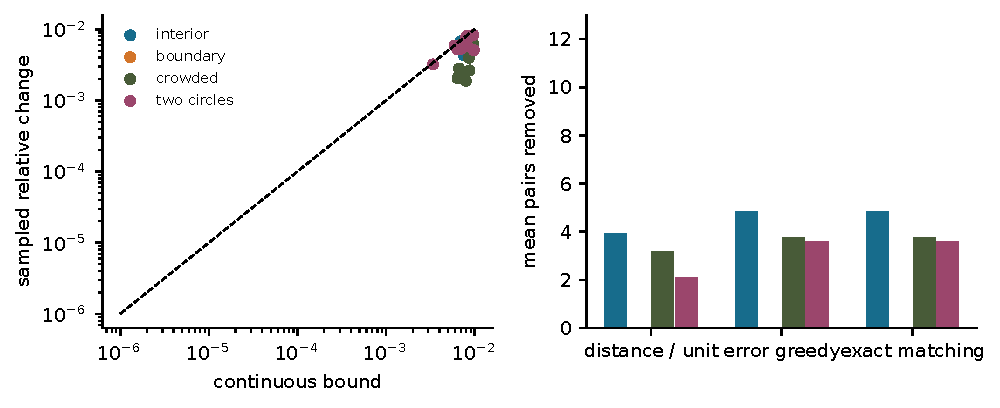
\includegraphics[width=\linewidth]{figures/banks.pdf}
\caption{Manufactured banks at budget $0.01$. Left: sampled change versus the continuous certificate, with the diagonal marking equality; zero-removal cases are omitted from the logarithmic plot. Right: mean removal counts. Gain optimization supplies most of the benefit at this budget; exact matching and error-greedy counts agree.}\label{fig:banks}
\end{figure}

\subsection{Noisy AAA-generated inputs}
We sample $\exp z$, $\log(2+z)$ on its principal branch, and $\tan(0.8z)$ at 512 roots of unity. Independent complex Gaussian perturbations have total variance $\sigma^2$, with $\sigma\in\{10^{-7},10^{-10},10^{-13}\}$. Four seeds per function and noise scale produce 36 cases. AAA is deliberately run with tolerance $10^{-14}$, at most 28 support points, and cleanup disabled. This overfitting setting stresses cleanup; it is not a recommendation for normal AAA use.

The nominal factored model uses the computed poles and zeros as exact dyadics and an anchor value at $1.234+0.234i$ to set its constant. We protect circles of radii $1$ and $1.1$ and use $E=0.01$. Its dense-grid disagreement with the original barycentric model, normalized by the latter's sampled maximum magnitude, ranges from $2.51\times10^{-13}$ to $1.87\times10^{-11}$. This is a diagnostic, not a factorization certificate.

The procedure removes 20--23 of the 27 poles in these fits: a 74.1--85.2\% reduction of the declared pole count. Table~\ref{tab:aaa} reports medians across the twelve cases at each noise scale. A separate SciPy comparator refits after support cleanup with \texttt{clean\_up\_tol=1e-7}. It is reported at a fixed setting and is not tuned to equal deletion counts or our relative-error budget. Its remaining pole count has medians $26$, $7$, and $8.5$ over the three noise scales, respectively; this comparison does not establish dominance of either method.

\begin{table}[t]\centering\small
\caption{AAA-generated nominal models: medians over twelve cases per noise scale. Absolute target errors are sampled over both circles; they are distinct from the relative compression contract.}\label{tab:aaa}
\begin{tabular}{lrrrrr}\toprule
Noise & Removed & Bound & Measured change & Target error before & Target error after\\\midrule
$10^{-7}$ & 23 & $4.49\!\times\!10^{-5}$ & $2.41\!\times\!10^{-5}$ & $9.04\!\times\!10^{-6}$ & $2.17\!\times\!10^{-5}$\\
$10^{-10}$ & 21 & $4.41\!\times\!10^{-8}$ & $2.66\!\times\!10^{-8}$ & $5.26\!\times\!10^{-9}$ & $2.49\!\times\!10^{-8}$\\
$10^{-13}$ & 20 & $9.82\!\times\!10^{-7}$ & $9.77\!\times\!10^{-7}$ & $8.09\!\times\!10^{-12}$ & $2.31\!\times\!10^{-6}$\\\bottomrule
\end{tabular}
\end{table}

Only three of the 36 reductions improve sampled error to the underlying analytic function. Particularly at the lowest noise, a permissive $1\%$ compression budget can discard information that was accurately fitted. This is expected from the objective: it optimizes certified degree removal, not denoising or target accuracy. If a separate approximation guarantee $\|r-f\|_K\le\eta$ is known, then the elementary absolute estimate
\begin{equation}
 \|\widetilde r-f\|_K\le\eta+E\|r\|_K\label{eq:target}
\end{equation}
can allocate the compression tolerance. In the absence of a validated $\eta$ and norm bound, \eqref{eq:target} is conditional.

\begin{figure}[t]\centering
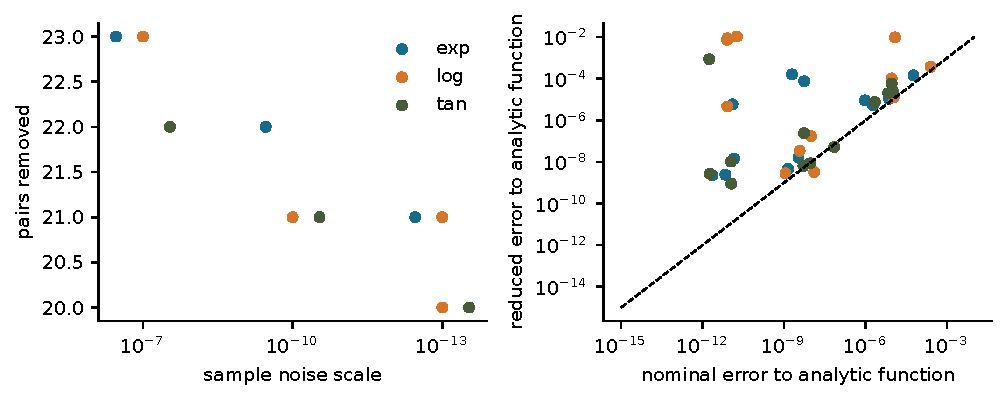
\includegraphics[width=\linewidth]{figures/aaa.pdf}
\caption{AAA-generated inputs. Left: cancellations for three analytic functions under the same $0.01$ budget. Right: sampled absolute error to the analytic target before and after compression. Points above the diagonal expose the cost of a compression objective that does not attempt denoising.}\label{fig:aaa}
\end{figure}

\subsection{Cost and reproducibility}
For random sparse candidate graphs, exact matching with 16, 32, and 64 zeros and poles takes approximately $0.003$, $0.020$, and $0.15$ seconds per full cardinality path (three runs per size). The graph density is approximately $15\%$ plus mandatory diagonal edges; detailed counts and timings are retained. These timings exclude geometric gain optimization and are not large-scale solver benchmarks. The complete declared experiment script, including figure generation, runs in about six seconds in the recorded environment, after dependency installation and font-cache initialization.

\section{Practical use and limitations}
The immediate application is an auditable cleanup stage for scalar rational surrogates. A simulation or approximation service can specify protected circles and a tolerance, receive a reduced factorization and a machine-readable certificate, and replay the decision without the optimizer. This can be useful when compact rational models are shipped to another team or evaluated repeatedly. Existing electromagnetic fitting workflows and commercial pole-zero simplification establish a practical setting for cleanup \cite{yuan,minreal}; our synthetic tests do not establish customer demand, patentability, or production performance.

Several limitations affect interpretation. First, circles are the protected sets. Covering a general contour by circles is not automatically equivalent, and a bound on a contour is not an interior bound unless the quotient is analytic there. Second, complex gains and independent pair removal do not enforce real symmetry, passivity, internal stability, or a prescribed state-space realization. Such requirements need additional constraints or grouped deletions. Third, high-degree root extraction can be ill-conditioned. The exact checker protects the declared factored model; it does not erase the conversion issue documented above.

Fourth, the product bound can be conservative when errors cancel in phase. Our matching is optimal within that compositional contract, rather than over all reduced rational functions. The gain optimizer is numerical; exact replay proves feasibility, not exact optimality of its gain proposal. Finally, the engineering experiments use analytic test functions and manufactured root banks, not measured scattering data or a production solver. Larger and independently sourced datasets are needed before making application-level performance claims.

\section{Conclusion}
Pole-zero cancellation admits a precise, continuous relative-error contract when the evaluation geometry is declared. On a circle, its local error is available in closed form. On several circles, individually safe normalizations can be incompatible, exactly when the convex hull of their image disks contains the origin. Verified pair errors compose into a rational product budget, and standard matching machinery can optimize that budget without floating-point logarithmic comparisons. The resulting implementation separates candidate generation from an independent acceptance check. The computational evidence supports this error-contract interpretation and also demonstrates its limits: safe compression need not improve approximation to the original function.

\section*{Data and code availability}
\texttt{CircleCancel} includes the gain proposer, exact matching, independent verifier, all experiment generators, raw CSV results, JSON certificates, figure sources, and this manuscript at \url{https://github.com/shi1720/circlecancel}. The verifier requires only Python's standard library; experiments additionally require the packages listed in the repository. All research claims refer to the stated mathematical model and the recorded experiments.

\begin{thebibliography}{10}\small
\bibitem{aaa} Y.~Nakatsukasa, O.~S\`ete, and L.~N.~Trefethen. The AAA algorithm for rational approximation. \emph{SIAM Journal on Scientific Computing}, 40(3):A1494--A1522, 2018. \href{https://doi.org/10.1137/16M1106122}{doi:10.1137/16M1106122}.
\bibitem{beckermann} B.~Beckermann, G.~Labahn, and A.~C.~Matos. On rational functions without Froissart doublets. arXiv:1605.00506, 2016. \url{https://arxiv.org/abs/1605.00506}.
\bibitem{continuation} L.~N.~Trefethen. Numerical analytic continuation. \emph{Japan Journal of Industrial and Applied Mathematics}, 40:1587--1636, 2023. \href{https://doi.org/10.1007/s13160-023-00599-2}{doi:10.1007/s13160-023-00599-2}.
\bibitem{yuan} H.~Yuan, J.~Ren, Y.~Li, and X.~Huang. Removing the Froissart doublets in a rational interpolation based on Loewner matrix. \emph{Applied Computational Electromagnetics Society Journal}, 38(1):60--66, 2023. \href{https://doi.org/10.13052/2023.ACES.J.380109}{doi:10.13052/2023.ACES.J.380109}.
\bibitem{boyd} S.~Boyd and L.~Vandenberghe. \emph{Convex Optimization}. Cambridge University Press, 2004. \url{https://web.stanford.edu/~boyd/cvxbook/}.
\bibitem{flows} R.~K.~Ahuja, T.~L.~Magnanti, and J.~B.~Orlin. \emph{Network Flows: Theory, Algorithms, and Applications}. Prentice Hall, 1993.
\bibitem{cvxpy} S.~Diamond and S.~Boyd. CVXPY: A Python-embedded modeling language for convex optimization. \emph{Journal of Machine Learning Research}, 17(83):1--5, 2016. \url{https://www.jmlr.org/papers/v17/15-408.html}.
\bibitem{scipy} P.~Virtanen et al. SciPy 1.0: fundamental algorithms for scientific computing in Python. \emph{Nature Methods}, 17:261--272, 2020. \href{https://doi.org/10.1038/s41592-019-0686-2}{doi:10.1038/s41592-019-0686-2}.
\bibitem{scipydoc} SciPy developers. \texttt{scipy.interpolate.AAA}: API reference and cleanup notes. Accessed 17 October 2026. \url{https://docs.scipy.org/doc/scipy/reference/generated/scipy.interpolate.AAA.html}.
\bibitem{minreal} MathWorks. Pole-zero simplification. Control System Toolbox documentation, R2026b. Accessed 17 October 2026. \url{https://www.mathworks.com/help/control/ug/pole-zero-simplification.html}.
\end{thebibliography}
\end{document}
